\documentclass{article}

\usepackage{amsmath,amssymb}
\usepackage{tikz}
\usepackage{pgfplots}
\usepackage{xcolor}
\usepackage[left=2.1cm,right=3.1cm,bottom=3cm,footskip=0.75cm,headsep=0.5cm]{geometry}
\usepackage{enumerate}
\usepackage{enumitem}
\usepackage{marvosym}
\usepackage{tabularx}
\usepackage{tikz-qtree}
\usetikzlibrary{patterns,arrows,calc,decorations.pathmorphing,backgrounds, positioning,fit,petri,decorations.fractals,trees,cd,automata,babel,shapes.geometric,arrows.meta,bending}

\usepackage[utf8]{inputenc}

\renewcommand*{\arraystretch}{1.4}

\newcolumntype{L}[1]{>{\raggedright\arraybackslash}p{#1}}
\newcolumntype{R}[1]{>{\raggedleft\arraybackslash}p{#1}}
\newcolumntype{C}[1]{>{\centering\let\newline\\\arraybackslash\hspace{0pt}}m{#1}}

\title{\textbf{Steuertheorie, Hausaufgabe 2}}
\author{\textsc{Henry Haustein}}
\date{}

\begin{document}
	\maketitle
	
	\section*{Aufgabe 1}
	\begin{enumerate}[label=(\alph*)]
		\item unelastische Nachfrage: Da die Produzentenrente von und nach Besteuerung gleich ist, tragen die Konsumenten die Steuer.
		\begin{center}
			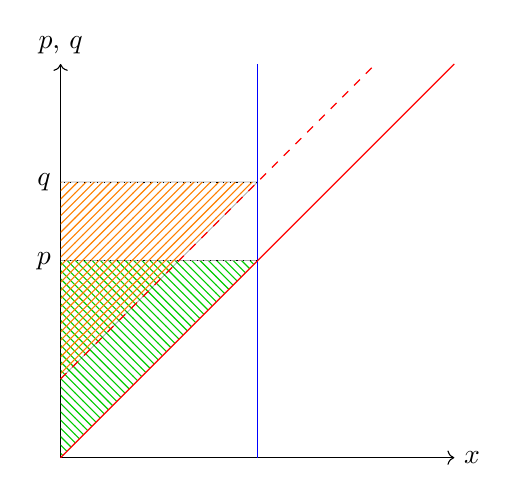
\begin{tikzpicture}
				\draw[->] (0,0) -- (5,0) node[right] {$x$};
				\draw[->] (0,0) -- (0,5) node[above] {$p$, $q$};
				
				\draw[pattern=north west lines, pattern color=green!80!black,ultra thin] (0,0) -- (2.5,2.5) -- (0,2.5) -- (0,0);
				\draw[pattern=north east lines, pattern color=orange, ultra thin] (0,1) -- (2.5,3.5) -- (0,3.5) -- (0,1);
				
				\draw[blue] (2.5,0) -- (2.5,5);
				\draw[red] (0,0) -- (5,5);
				\draw[red,dashed] (0,1) -- (4,5);
				
				\draw[dotted] (2.5,2.5) -- (0,2.5) node[left] {$p$};
				\draw[dotted] (2.5,3.5) -- (0,3.5) node[left] {$q$};
				
			\end{tikzpicture} \\
			\textcolor{blue}{Nachfrage}, \textcolor{red}{Angebot ohne/mit Steuern}, \textcolor{green!80!black}{Produzentenrente ohne Besteuerung}, \textcolor{orange}{Produzentenrente nach Besteuerung}
		\end{center}
		elastische Nachfrage: Da die Produzentenrente sich durch die Besteuerung verringert, tragen die Produzenten die Steuer.
		\begin{center}
			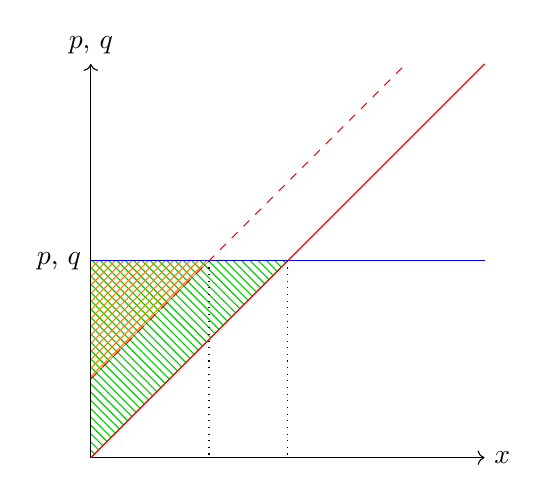
\begin{tikzpicture}
				\draw[->] (0,0) -- (5,0) node[right] {$x$};
				\draw[->] (0,0) -- (0,5) node[above] {$p$, $q$};
				
				\draw[pattern=north west lines, pattern color=green!80!black,ultra thin] (0,0) -- (2.5,2.5) -- (0,2.5) -- (0,0);
				\draw[pattern=north east lines, pattern color=orange, ultra thin] (0,1) -- (1.5,2.5) -- (0,2.5) -- (0,1);
				
				\draw[blue] (0,2.5) -- (5,2.5);
				\draw[red] (0,0) -- (5,5);
				\draw[red,dashed] (0,1) -- (4,5);
				
				\draw[dotted] (2.5,2.5) -- (0,2.5) node[left] {$p$, $q$};
				\draw[dotted] (1.5,2.5) -- (1.5,0);
				\draw[dotted] (2.5,2.5) -- (2.5,0);
				
			\end{tikzpicture} \\
			\textcolor{blue}{Nachfrage}, \textcolor{red}{Angebot ohne/mit Steuern}, \textcolor{green!80!black}{Produzentenrente ohne Besteuerung}, \textcolor{orange}{Produzentenrente nach Besteuerung}
		\end{center}
		\item unelastisches Angebot: Da die Konsumentenrente von und nach Besteuerung gleich ist, tragen die Produzenten die Steuer.
		\begin{center}
			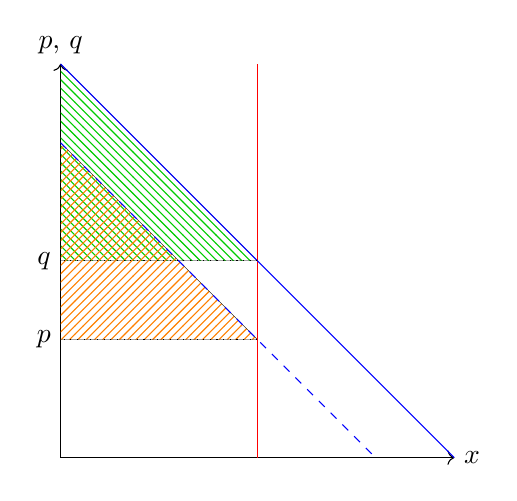
\begin{tikzpicture}
				\draw[->] (0,0) -- (5,0) node[right] {$x$};
				\draw[->] (0,0) -- (0,5) node[above] {$p$, $q$};
				
				\draw[pattern=north west lines, pattern color=green!80!black,ultra thin] (0,5) -- (2.5,2.5) -- (0,2.5) -- (0,5);
				\draw[pattern=north east lines, pattern color=orange, ultra thin] (0,4) -- (2.5,1.5) -- (0,1.5) -- (0,4);
				
				\draw[red] (2.5,0) -- (2.5,5);
				\draw[blue] (0,5) -- (5,0);
				\draw[blue,dashed] (0,4) -- (4,0);
				
				\draw[dotted] (2.5,1.5) -- (0,1.5) node[left] {$p$};
				\draw[dotted] (2.5,2.5) -- (0,2.5) node[left] {$q$};
				
			\end{tikzpicture} \\
			\textcolor{blue}{Nachfrage ohne/mit Steuern}, \textcolor{red}{Angebot}, \textcolor{green!80!black}{Konsumentenrente ohne Besteuerung}, \textcolor{orange}{Konsumentenrente nach Besteuerung}
		\end{center}
		elastisches Angebot: Da die Konsumentenrente sich durch die Besteuerung verringert, tragen die Konsumenten die Steuer.
		\begin{center}
			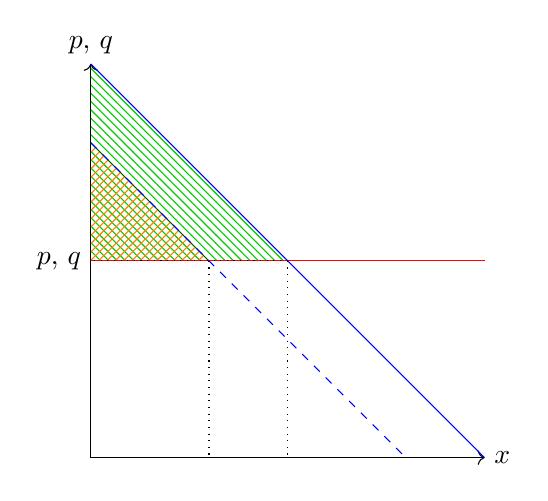
\begin{tikzpicture}
				\draw[->] (0,0) -- (5,0) node[right] {$x$};
				\draw[->] (0,0) -- (0,5) node[above] {$p$, $q$};
				
				\draw[pattern=north west lines, pattern color=green!80!black,ultra thin] (0,5) -- (2.5,2.5) -- (0,2.5) -- (0,5);
				\draw[pattern=north east lines, pattern color=orange, ultra thin] (0,4) -- (1.5,2.5) -- (0,2.5) -- (0,4);
				
				\draw[red] (0,2.5) -- (5,2.5);
				\draw[blue] (0,5) -- (5,0);
				\draw[blue,dashed] (0,4) -- (4,0);
				
				\draw[dotted] (2.5,2.5) -- (0,2.5) node[left] {$p$, $q$};
				\draw[dotted] (1.5,2.5) -- (1.5,0);
				\draw[dotted] (2.5,2.5) -- (2.5,0);
				
			\end{tikzpicture} \\
			\textcolor{blue}{Nachfrage ohne/mit Steuern}, \textcolor{red}{Angebot}, \textcolor{green!80!black}{Konsumentenrente ohne Besteuerung}, \textcolor{orange}{Konsumentenrente nach Besteuerung}
		\end{center}
	\end{enumerate}

	\section*{Aufgabe 2}
	\begin{enumerate}[label=(\alph*)]
		\item Diagramm
		\begin{center}
			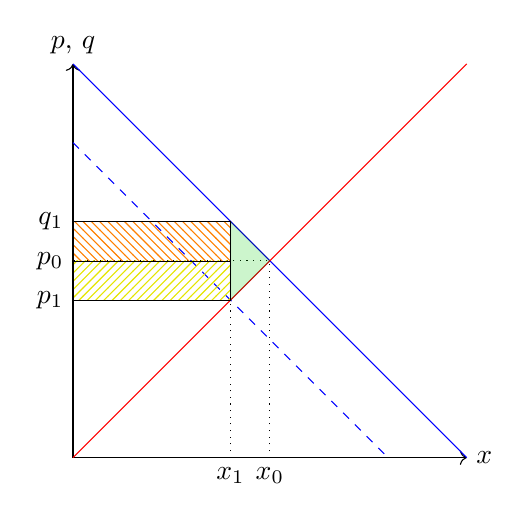
\begin{tikzpicture}
				\draw[->] (0,0) -- (5,0) node[right] {$x$};
				\draw[->] (0,0) -- (0,5) node[above] {$p$, $q$};
				
				\draw[blue] (0,5) -- (5,0);
				\draw[blue,dashed] (0,4) -- (4,0);
				\draw[red] (0,0) -- (5,5);
				
				\draw[dotted] (2.5,0) node[below] {$x_0$} -- (2.5,2.5) -- (0,2.5) node[left] {$p_0$};
				
				\draw[dotted] (2,0) node[below] {$x_1$} -- (2,2) -- (0,2) node[left] {$p_1$};
				\draw[dotted] (2,2) -- (2,3) -- (0,3) node[left] {$q_1$};
				
				\draw[fill=green!80!black,opacity=0.2] (2,2) -- (2.5,2.5) -- (2,3) -- (2,2);
				
				\draw[pattern=north west lines, pattern color=orange,ultra thin] (0,3) rectangle (2,2.5);
				\draw[pattern=north east lines, pattern color=yellow!90!black,ultra thin] (0,2) rectangle (2,2.5);
				
			\end{tikzpicture} \\
			\textcolor{blue}{Nachfrage ohne/mit Steuern}, \textcolor{red}{Angebot}, \textcolor{green!80!black}{Wohlfahrtsverlust}, \textcolor{yellow!90!black}{Traglast Produzenten}, \textcolor{orange}{Traglast Konsumenten}
		\end{center}
		\item Es gilt
		\begin{align}
			GZB - t &= GK \notag \\
			a-bx - t &= x \notag \\
			a-t &= (b+1)x \notag \\
			x_1 &= \frac{a-t}{b+1} \notag
		\end{align}
		Der Nettopreis ist dann $p_1=GK(x_1)=\frac{a-t}{b+1}$ und der Bruttopreis $q_1=p_1+t= \frac{a-t}{b+1}+t$
		\item Es gilt
		\begin{align}
			\frac{GZB}{1+\theta} &= GK \notag \\
			\frac{a-bx}{1+\theta} &= x \notag \\
			a-bx &= (1+\theta)x \notag \\
			a &= (1+b+\theta)x \notag \\
			x_2 &= \frac{a}{1+b+\theta} \notag
		\end{align}
		\item Das Steueraufkommen ist
		\begin{align}
			T &= x_1\cdot t \notag \\
			&= \frac{at-t^2}{b+1} \notag \\
			\frac{\partial T}{\partial t} &= \frac{a-2t}{b+1} \notag
		\end{align}
		\item Das Steueraufkommen wird dann maximal, wenn $a=2t$, also $t=\frac{a}{2}$. Bei geringerem oder höherem Steuersatz wird das Steueraufkommen sinken.
		\item Traglast der Konsumenten:
		\begin{align}
			(q_1-p_0)\cdot x_1 &= \frac{a-t}{1+b}\left(\frac{a+bt}{1+b}-\frac{a}{1+b}\right) \notag \\
			&= \frac{bt}{1+b}\cdot\frac{a-t}{1+b} \notag \\
			&= \frac{abt - bt^2}{(1+b)^2} \notag \\
			&= \frac{b(at-t^2)}{(1+b)^2} \notag
		\end{align}
		Traglast der Produzenten
		\begin{align}
			(p_0-p_1)\cdot x_1 &= \frac{a-t}{1+b}\left(\frac{a}{1+b}-\frac{a-t}{1+b}\right) \notag \\
			&= \frac{t}{1+b}\cdot\frac{a-t}{1+b} \notag \\
			&= \frac{at-t^2}{(1+b)^2} \notag
		\end{align}
	\end{enumerate}

	\section*{Aufgabe 3}
	\begin{enumerate}[label=(\alph*)]
		\item Es gilt
		\begin{align}
			GZB &= GK+t \notag \\
			12-x &= \frac{x}{2} + 3 \notag \\
			9 &= \frac{3}{2}x \notag \\
			x &= 6 \notag
		\end{align}
		Der Nettopreis ist dann $p=Gk(6)=3$ und der Bruttopreis ist dann $q=GZB(6)=6$.
		\item Das Steueraufkommen ist $T=x\cdot t = 6\cdot 3=18$.
		\item Bei einer Wertsteuer gilt
		\begin{align}
			GZB &= (1+\theta)GK \notag \\
			12-x &= (1+\theta)\frac{x}{2} \notag \\
			12 &= (3+\theta)\frac{x}{2} \notag \\
			x &= \frac{24}{3+\theta} \notag
		\end{align}
		Der Nettopreis ist dann $p=GK\left(\frac{24}{3+\theta}\right)=\frac{12}{3+\theta}$ und der Bruttopreis ist $q=GZB\left(\frac{24}{3+\theta}\right)=\frac{12(1+\theta)}{3+\theta}$. Für das Steueraufkommen gilt dann
		\begin{align}
			T &= x\cdot \theta \cdot p \notag \\
			18 &= \frac{24}{3+\theta}\cdot\theta\cdot\frac{12}{3+\theta} \notag \\
			\theta &= 1 \notag
		\end{align}
		und mit $\tau=\frac{\theta}{1+\theta}$ folgt $\tau=\frac{1}{2}$.
		\item Aufkommensneutrale Mengen- und Wertsteuern verändern die Preise und Mengen nicht (gilt nur bei vollständiger Konkurrenz!) $\Rightarrow$ der Wohlfahrtsverlust ist bei allen identisch.
	\end{enumerate}

	\section*{Aufgabe 4}
	\begin{enumerate}[label=(\alph*)]
		\item Der Monopolist maximiert seinen Gewinn:
		\begin{align}
			\Pi_\theta &= x\cdot p(x) - K(x) \notag \\
			&= x\cdot \frac{q(x)}{1+\theta} - K(x) \notag \\
			&= \frac{120x-x^2}{2} - \frac{x^2}{2} \notag \\
			&= 60x - x^2 \notag
		\end{align}
		Also
		\begin{align}
			\frac{\partial\Pi_\theta}{\partial x} &= 60-2x = 0 \notag \\
			x_\theta &= 30 \notag
		\end{align}
		Der Bruttopreis ist dann $q=GZB(x)=120-30=90$ und der Nettopreis $p=\frac{q}{1+\theta}=\frac{90}{2}=45$.
		\item Das Steueraufkommen ist $T=x\cdot p\cdot\theta=30\cdot 45\cdot 1 = 1350$.
		\item Bei einer Mengensteuer maximiert der Monopolist auch seinen Gewinn:
		\begin{align}
			\Pi_t &= x\cdot p(x) - K(x) \notag \\
			&= x(q(x) - t) - K(x) \notag \\
			&= 120x-x^2-tx - \frac{x^2}{2} \notag \\
			&= 120x-tx - \frac{3}{2}x^2 \notag
		\end{align}
		Also
		\begin{align}
			\frac{\partial\Pi_t}{\partial x} &= 120-t-3x = 0 \notag \\
			3x &= 120-t \notag \\
			x_t &= 40-\frac{t}{3} \notag
		\end{align}
		Da $x_\theta=x_t=30=40-\frac{t}{3}$ $\Rightarrow$ $t=30$.
		\item Das Steueraufkommen ist $T=x_t\cdot t = 30\cdot 30=900$.
		\item Das Steueraufkommen ist $T=x_t\cdot t=40t-\frac{t^2}{3}$. Es gilt
		\begin{align}
			\frac{\partial T}{\partial t} &= 40-\frac{2}{3}t =0 \notag \\
			t^\ast &= 60 \notag
		\end{align}
		Bei einer Steuer von $t=60$ wird das Steueraufkommen maximal, bei einer niedrigeren oder höheren Steuer sinkt das Steueraufkommen.
	\end{enumerate}

	\section*{Aufgabe 5}
	\begin{enumerate}[label=(\alph*)]
		\item Diagramm
		\begin{center}
			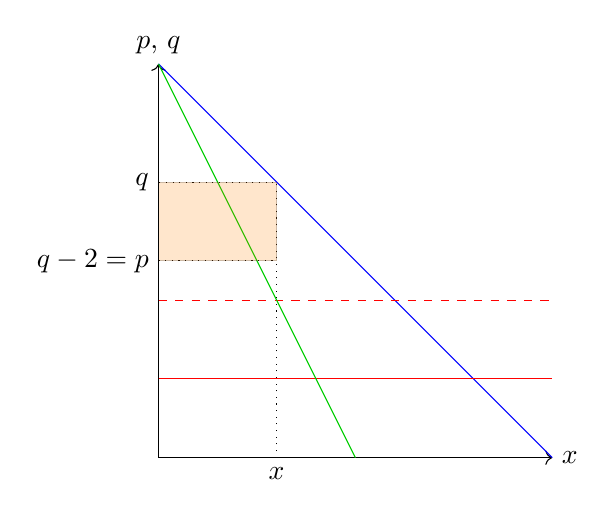
\begin{tikzpicture}
				\draw[->] (0,0) -- (5,0) node[right] {$x$};
				\draw[->] (0,0) -- (0,5) node[above] {$p$, $q$};
				
				\draw[blue] (0,5) -- (5,0);
				\draw[red] (0,1) -- (5,1);
				\draw[red,dashed] (0,2) -- (5,2);
				\draw[green!80!black] (0,5) -- (2.5,0);
				
				\draw[dotted] (1.5,0) node[below] {$x$} -- (1.5,3.5) -- (0,3.5) node[left] {$q$};
				\draw[dotted] (0,2.5) node[left] {$q-2=p$} -- (1.5,2.5);
				
				\draw[fill=orange,opacity=0.2] (0,3.5) rectangle (1.5,2.5);
			\end{tikzpicture} \\
			\textcolor{blue}{GZB}, \textcolor{red}{Grenzkosten ohne/mit Steuern}, \textcolor{green!80!black}{Grenzerlös}, \textcolor{orange}{Steueraufkommen}
		\end{center}
		\item Der Monopolist maximiert seinen Gewinn, also
		\begin{align}
			\Pi &= x\cdot p(x) - C(x) \notag \\
			\label{amoroso}
			&= x(GZB(x) - t) - C(x) \tag{\textasteriskcentered} \\
			&= 10x-x^2-2x-2x \notag \\
			&= 6x-x^2 \notag
		\end{align}
		Also
		\begin{align}
			\frac{\partial\Pi}{\partial x} &= 6-2x = 0 \notag \\
			x &= 3 \notag
		\end{align}
		Der Bruttopreis ist $q=GZB(3)=7$ und der Nettopreis $p=q-2=5$. Das Steueraufkommen ist $T=x\cdot t=3\cdot 2=6$.
		
		Ausgehend von \eqref{amoroso} kann man ableiten, dass im Gleichgewicht gilt
		\begin{align}
			GZB + GZB'\cdot x = GK + t \notag
		\end{align}
		mit $\eta=\frac{\partial x}{\partial GZB}\cdot\frac{GZB}{x}$ folgt
		\begin{align}
			GZB + \frac{1}{\eta}GZB &= GK + t \notag
		\end{align}
		$\Rightarrow$ Amoroso-Robinson-Relation
		\item Wie man in Aufgabe 4 sieht, ist bei einer Wertsteuer im Monopol das Steueraufkommen größer als bei einer Mengensteuer.
	\end{enumerate}

	\section*{Aufgabe 6}
	\begin{enumerate}[label=(\alph*)]
		\item Es gilt $x(q)=q^\eta$ und deshalb $q(x)=\sqrt[\eta]{x}$. Der Monopolist hat einen Gewinn von $\Pi=x\cdot q(x) - tx - K(x)$ und maximiert diesen:
		\begin{align}
			\frac{\partial\Pi}{\partial x} &= q(x) + x\cdot q'(x) - t - GK(x) = 0 \notag \\
			0 &= \sqrt[\eta]{x} + x\cdot\frac{1}{\eta}\cdot x^{\frac{1}{\eta}-1} - t - c \notag \\
			t+c &= \sqrt[\eta]{x} + \frac{1}{\eta}\sqrt[\eta]{x} \notag \\
			t+c &= \sqrt[\eta]{x} + \left(1+\frac{1}{\eta}\right) \notag \\
			t+c &= q\left(1+\frac{1}{\eta}\right) \notag \\
			q &= \frac{t+c}{1+\frac{1}{\eta}} \notag
		\end{align}
		\item Es gilt
		\begin{align}
			\frac{dq}{dt} &= \frac{1}{1+\frac{1}{\eta}} = 2 \notag \\
			1+\frac{1}{\eta} &= \frac{1}{2} \notag \\
			\eta &= -2 \notag
		\end{align}
		\item Es gilt
		\begin{align}
			V = \frac{\Pi}{T} &= \frac{x\cdot q(x) - tx - \overbrace{K(x)}^{cx}}{tx} \notag \\
			&= \frac{q(x)-t-c}{t} \notag \\
			&= \frac{\frac{c+t}{1+\frac{1}{\eta}} - (c+t)}{t} \notag
		\end{align}
		\item Es gilt
		\begin{align}
			\frac{\partial V}{\partial t} &= \frac{c}{(\eta+1)t^2} < 0 \notag
		\end{align}
	\end{enumerate}
	
\end{document}